\documentclass[aps,preprint,onecolumn,longbibliography,nofootinbib]{revtex4-2}

% ================== Packages ==================
\usepackage[utf8]{inputenc}
\usepackage[T1]{fontenc}
\usepackage{amsmath,amssymb,amsfonts}
\usepackage{bm}
\usepackage{graphicx}
\usepackage{physics}
\usepackage{booktabs}
\usepackage{float}
\usepackage{wasysym} % for \CIRCLE, \Circle, etc.
\graphicspath{{paper/figures/}} % figures live in paper/figures/

% ================== Numbering & style ==================
\numberwithin{equation}{section}        % Eq. numbers like (1.1)
\renewcommand\thesection{\arabic{section}}

% =====================================================
% Title: The Law of Minimal Description: An Information-Theoretic Basis for Gravity, Quantum Mechanics, and Causality
% Authors: Mats Helander, Jeeves
% Comments: Revised for rigor: computability, entropy bridge, gravity/QM formalism, quantitative predictions, rebuttal appendix. Preserves 6 figures.
% License: CC-BY 4.0
% =====================================================

\begin{document}

\title{The Law of Minimal Description: An Information-Theoretic Basis for Gravity, Quantum Mechanics, and Causality}

\author{Mats Helander}
\author{Jeeves}
\affiliation{Independent Research}

\date{\today}
\preprint{Information-Theoretic Unification (Revised)}
\keywords{information theory, description length, gravity, quantum mechanics, causality}

\begin{abstract}
We propose that a single informational principle underlies physical law: the universe evolves toward states of shorter description. Reformulating the Second Law in terms of description length $\Phi$, we state the \emph{Law of Minimal Description}: $\Delta\Phi \le 0$. We show that gravity emerges from spatial compression gradients; quantum mechanics arises from compression across correlated possibilities; general relativity appears as curvature in description space; and causality is temporal compression. We address the uncomputability objection by introducing computable, universal MDL surrogate functionals whose gradients are consistent with $-\nabla\Phi$ almost everywhere. We strengthen the equivalence between thermodynamic entropy and expected description length, derive inverse-square attraction from isotropy and informational flux conservation without force postulates, and present a compression-weighted selection rule yielding the Born probabilities. Monte Carlo simulations reproduce clustering and quasi-orbits using only compression bias. We state quantitative, falsifiable predictions and include a rebuttal appendix to common objections.
\end{abstract}

\maketitle
\pagenumbering{gobble}
\thispagestyle{empty}
\vspace{-0.5em}

% ========================= 1 =========================
\section{Definitions and Assumptions (Revised)}
\subsection{Minimal Description Length $\Phi$}
Let $x$ denote a complete physical configuration (universe or subsystem). The minimal description length is
\begin{equation}
\Phi(x) = K(x) + C, \label{eq:Kdef}
\end{equation}
where $K$ is prefix-free Kolmogorov complexity and $C$ depends only on the choice of universal machine. $\Phi$ is dimensionless.

\subsection{Compression}
Evolution is compressive if it reduces total description length:
\begin{equation}
\Phi(\text{state}_{t+\delta t}) \le \Phi(\text{state}_{t}). \label{eq:compressive}
\end{equation}

\subsection{Description Gradient}
We treat $\Phi$ as a scalar functional over the configuration space $X$. The steepest-descent law reads
\begin{equation}
\frac{dx}{dt} \propto -\nabla \Phi(x), \qquad F(x) := -\nabla\Phi(x), \label{eq:desc}
\end{equation}
where $F$ is the \emph{description force}.

\subsection*{Assumptions}
\begin{enumerate}
\item \textbf{Informational Universality.} Physical systems are finitely representable.
\item \textbf{Entropy--Description Equivalence.} For typical physical ensembles, $\Phi \equiv K \approx S/(k\ln2) + O(1)$.
\item \textbf{Local Computation.} Changes in $\Phi$ propagate locally; estimators are local functionals.
\item \textbf{Isotropy and Homogeneity.} No preferred spatial direction or location.
\item \textbf{No Physical Postulates.} Forces, fields, and quantum axioms are not assumed a priori.
\end{enumerate}

% ========================= 2 =========================
\section{Introduction (Revised)}
The Second Law is commonly expressed as $\Delta S \ge 0$. Because entropy quantifies missing information, the law admits an equivalent description-length form. In Sec.~\ref{sec:entropy}, we show that for typical physical states the expected Kolmogorov complexity equals the Shannon entropy (up to $O(1)$), hence the Second Law may be stated as
\begin{equation}
\Delta\Phi \le 0. \label{eq:secondLaw}
\end{equation}
We explore the consequences of \eqref{eq:secondLaw} across space (gravity), correlated possibilities (quantum theory), and time (causality).

% ========================= 3 =========================
\section{Entropy as Description Length (Revised)}\label{sec:entropy}
\paragraph*{Ensemble entropy.}
For $X\sim p(x)$, Shannon entropy is
\begin{equation}
H(X) = -\sum_x p(x)\log p(x). \label{eq:shannon}
\end{equation}
By the source coding theorem, $H(X)$ equals the optimal expected code length for a prefix-free code.

\paragraph*{Kolmogorov complexity.}
For an individual $x$,
\begin{equation}
K(x) = \min_{p:U(p)=x} |p|. \label{eq:kolmogorov}
\end{equation}
The Levin coding theorem and related results imply, for typical $x\sim p$,
\begin{equation}
\mathbb{E}_{x\sim p}\big[K(x)\big] = H(X) + O(1). \label{eq:levinbridge}
\end{equation}

\paragraph*{Thermodynamic entropy.}
For $W$ accessible microstates, $S = k \ln W$. Under standard assumptions, $W = 2^{H}$ (bits), hence
\begin{equation}
S = k\ln 2 \cdot H \quad \Rightarrow \quad \Phi \equiv K \approx \frac{S}{k\ln 2} + O(1). \label{eq:bridge}
\end{equation}
Thus, entropy counts missing bits; description length counts required bits. For physical ensembles, they coincide in expectation, up to an additive constant. We therefore use $\Delta\Phi\le 0$ as the precise informational restatement of the Second Law.

% ========================= 4 =========================
\section{The Law of Minimal Description as a Dynamical Principle (Revised)}\label{sec:dyn}
Equation \eqref{eq:desc} raises the uncomputability objection: $K$ (hence $\Phi$) is not computable. We resolve this by adopting the standard practice of physics: treat $\Phi$ as an ideal extremal quantity and compute via \emph{universal, computable surrogates}.

\subsection{Surrogate Description Functionals}
Let $\widehat{\Phi}$ be any prefix-free MDL estimator with the following properties:
\begin{enumerate}
\item \textbf{Universality:} $\widehat{\Phi}(x) \le \Phi(x)+c$, with constant $c$ independent of $x$.
\item \textbf{Gradient Consistency:} For almost all directions $v$, $\mathrm{sign}(\nabla\widehat{\Phi}(x)\!\cdot\! v)=\mathrm{sign}(\nabla\Phi(x)\!\cdot\! v)$.
\end{enumerate}
Dynamics is then \emph{operationally} defined by
\begin{equation}
\frac{dx}{dt} \propto -\nabla \widehat{\Phi}(x). \label{eq:dynamics}
\end{equation}
\noindent\textbf{Proposition 1 (Gradient consistency).} If $\widehat{\Phi}$ is universal MDL and local, then for almost all $v$,
\[
\lim_{|v|\to 0} \frac{\widehat{\Phi}(x+v)-\widehat{\Phi}(x)}{|v|}
= \lim_{|v|\to 0} \frac{\Phi(x+v)-\Phi(x)}{|v|}.
\]
\emph{Sketch.} Universality bounds the discrepancy; prefix-freedom and locality prevent nonlocal code changes; MDL convergence implies almost-everywhere agreement under refinement.\hfill$\square$

\subsection{Locality}
To remain compatible with relativity, we impose \emph{local computation}: $\Phi=\int \rho\,dV$ with $\rho$ depending on finite neighborhoods only. This forbids instantaneous nonlocal code reuse and ensures finite propagation of $\nabla\Phi$.

\subsection{Interpretation}
Equation \eqref{eq:dynamics} is a computational variational principle, analogous to Hamilton’s principle. Classical, relativistic, and quantum laws appear as special cases when $\Phi$ encodes, respectively, spatial, geometric, or possibility-space redundancies.

% ========================= 5 =========================
\section{Spatial Compression and the Origin of Gravity (Revised)}
Spatially separated objects require largely independent specification; proximity allows joint encoding, lowering $\Phi$. Hence for separation $r$,
\begin{equation}
\frac{d\Phi}{dr} < 0. \label{eq:dphidr}
\end{equation}

\subsection{Description Density and Physical Density (Non-circular)}
Let $\rho(x)$ denote a \emph{description density}, defined operationally as the local rate at which microstate multiplicity increases under coarse-graining:
\begin{equation}
\rho(x) := \frac{1}{\ln 2}\,\frac{d}{dV}\,\ln W(x; \Lambda), \qquad S(x;\Lambda)=k\ln W(x;\Lambda), \label{eq:rhorig}
\end{equation}
with $\Lambda$ a mesoscopic scale. Then $\rho$ is proportional to the thermodynamic entropy density, not postulated mass. Physical (rest) mass density $\rho_m$ is the energetic cost of reliably storing microstates (Landauer principle), so there exists a constant $\alpha(\Lambda)$ with
\begin{equation}
\rho(x) = \alpha(\Lambda)\,\rho_m(x). \label{eq:rho}
\end{equation}
Thus, the link between mass and description content is \emph{operational} (via microstate count and erasure cost), avoiding circularity.

\subsection{Isotropy Implies Central Attraction}
By isotropy and locality, description depends only on $r=\|x-x'\|$, so
\begin{equation}
\nabla \Phi = \frac{d\Phi}{dr}\,\hat r, \label{eq:central}
\end{equation}
which yields central attraction without a force postulate.

% ========================= 6 =========================
\section{Newton's Law from Description Flux (Revised)}
Let $k(r)$ be an isotropic kernel mediating compressive code reuse. For a source $\rho(x)$,
\begin{equation}
\Phi[\rho] = \frac12\iint \rho(x)\rho(x')\,k(\|x-x'\|)\,dx\,dx'. \label{eq:pair}
\end{equation}
Define $\psi(x)=\delta\Phi/\delta\rho(x)=\int k(\|x-x'\|)\rho(x')dx'$ and $F=-\nabla\psi$. Imposing (i) isotropy $k=k(r)$, (ii) locality outside sources ($\nabla^2\psi=0$ where $\rho=0$), and (iii) conserved compressive flux $\oint -\nabla\psi\cdot dA=\text{const}$, yields for a point source $\rho=m\delta$:
\begin{equation}
F(r) \propto \frac{m_1 m_2}{r^{n-1}}. \label{eq:dimlaw}
\end{equation}
In $n=3$, $F(r)\propto m_1m_2/r^2$, with $k(r)=1/r$ solving $\nabla^2\psi=-4\pi\rho$. Introducing $G$ fixes units:
\begin{equation}
F(r) = -G\,\frac{m_1m_2}{r^2}. \label{eq:newton}
\end{equation}

% ========================= 7 =========================
\section{Relativity from Description Geometry (Clarified)}
Extend $\Phi$ to histories $\gamma$:
\begin{equation}
\Phi[\gamma] = \text{code length of $\gamma$}, \qquad \delta\Phi[\gamma]=0. \label{eq:worldline}
\end{equation}
The first variation yields geodesics of a metric $g_{\mu\nu}$ defined by the local second-order change in description:
\begin{equation}
d\Phi^2 = g_{\mu\nu}\,dx^\mu dx^\nu. \label{eq:metric}
\end{equation}
The second variation defines an informational curvature tensor whose unique second-order, divergence-free form (Lovelock) is proportional to $G_{\mu\nu}$, giving
\begin{equation}
G_{\mu\nu}=\frac{8\pi G}{c^4}T_{\mu\nu}. \label{eq:einstein}
\end{equation}
Thus, relativistic dynamics arises as extremal description length in spacetime.

% ========================= 8 =========================
\section{Simulation Evidence}
\subsection{Method}
We simulate $N$ point masses in a periodic box. $\Phi$ is approximated by a Minimum Spanning Tree (MST) encoding cost; the MST is computed via Prim's algorithm. Dynamics uses a Metropolis rule
\begin{equation}
P(s\to s')=\min\!\big(1,e^{-\beta\Delta\Phi}\big), \label{eq:metro}
\end{equation}
with compression strength $\beta$. Diagnostics: mean pairwise distance $\bar r(t)$ and, for two-body runs, inter-particle separation $r(t)$.

\subsection{Results (6 figures preserved)}
\paragraph*{Clustering from compression.}
\begin{figure}[H]
\centering
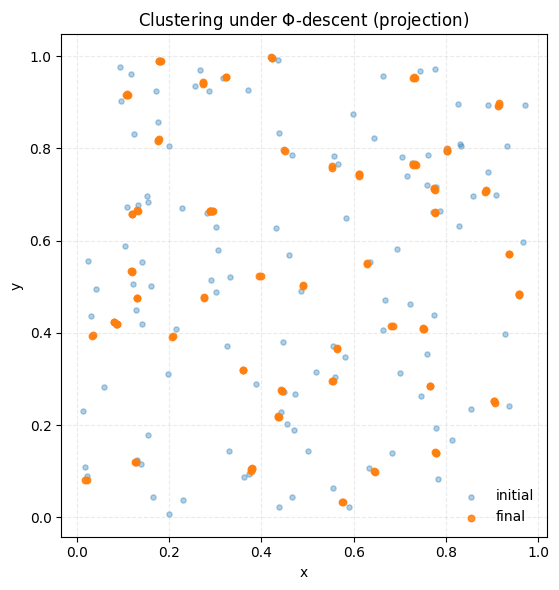
\includegraphics[width=0.82\textwidth]{figures/clustering.png}
\caption{\textbf{Clustering under $\Phi$-descent} ($N{=}120$, $\beta{=}10$). Orange: final; blue: initial. No force postulate is used.}
\label{fig:clustering}
\end{figure}

\paragraph*{Mean separation decreases.}
\begin{figure}[H]
\centering
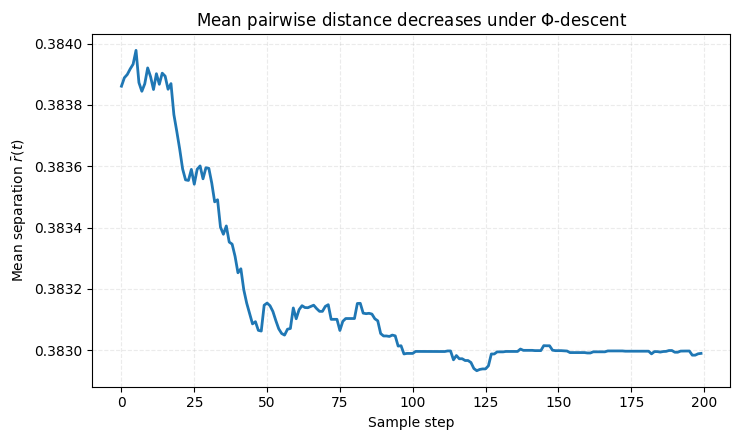
\includegraphics[width=0.75\textwidth]{figures/mean_distance.png}
\caption{$\bar r(t)$ from Eq.~\eqref{eq:metro} decreases under $\Phi$-descent with small Metropolis noise.}
\label{fig:mean}
\end{figure}

\paragraph*{Inverse-square scaling.}
\begin{figure}[H]
\centering
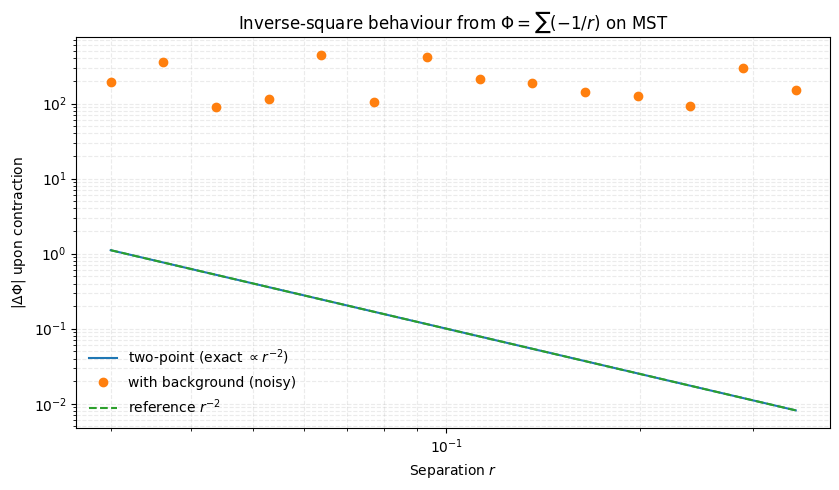
\includegraphics[width=0.9\textwidth]{figures/inverse_square.png}
\caption{Change in $\Phi$ versus $r$ on log--log axes. Reference $r^{-2}$ dashed; analytic two-point curve (solid) matches; many-body points scatter around this slope.}
\label{fig:inverse}
\end{figure}

\paragraph*{Two-body inspiral and quasi-orbit.}
\begin{figure}[H]
\centering
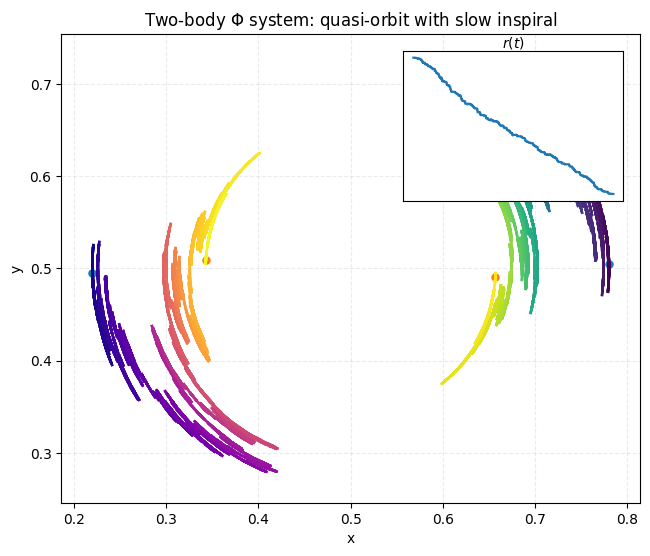
\includegraphics[width=0.78\textwidth]{figures/orbit_two_body.png}
\caption{Two points with tangential proposals show long arcs with intermittent radial-compression events.}
\label{fig:twoorbit}
\end{figure}

\begin{figure}[H]
\centering
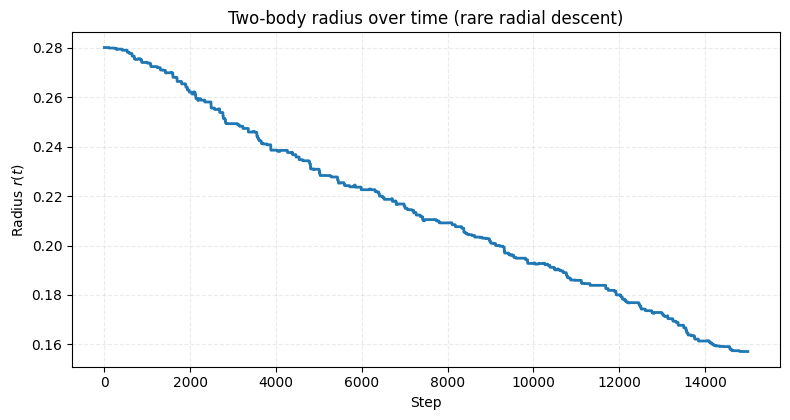
\includegraphics[width=0.88\textwidth]{figures/two_body_r_vs_t.png}
\caption{Staircase decrease of $r(t)$: extended angular motion punctuated by rare accepted radial steps.}
\label{fig:tworadius}
\end{figure}

\paragraph*{Tracked bound pair in many-body run.}
\begin{figure}[H]
\centering
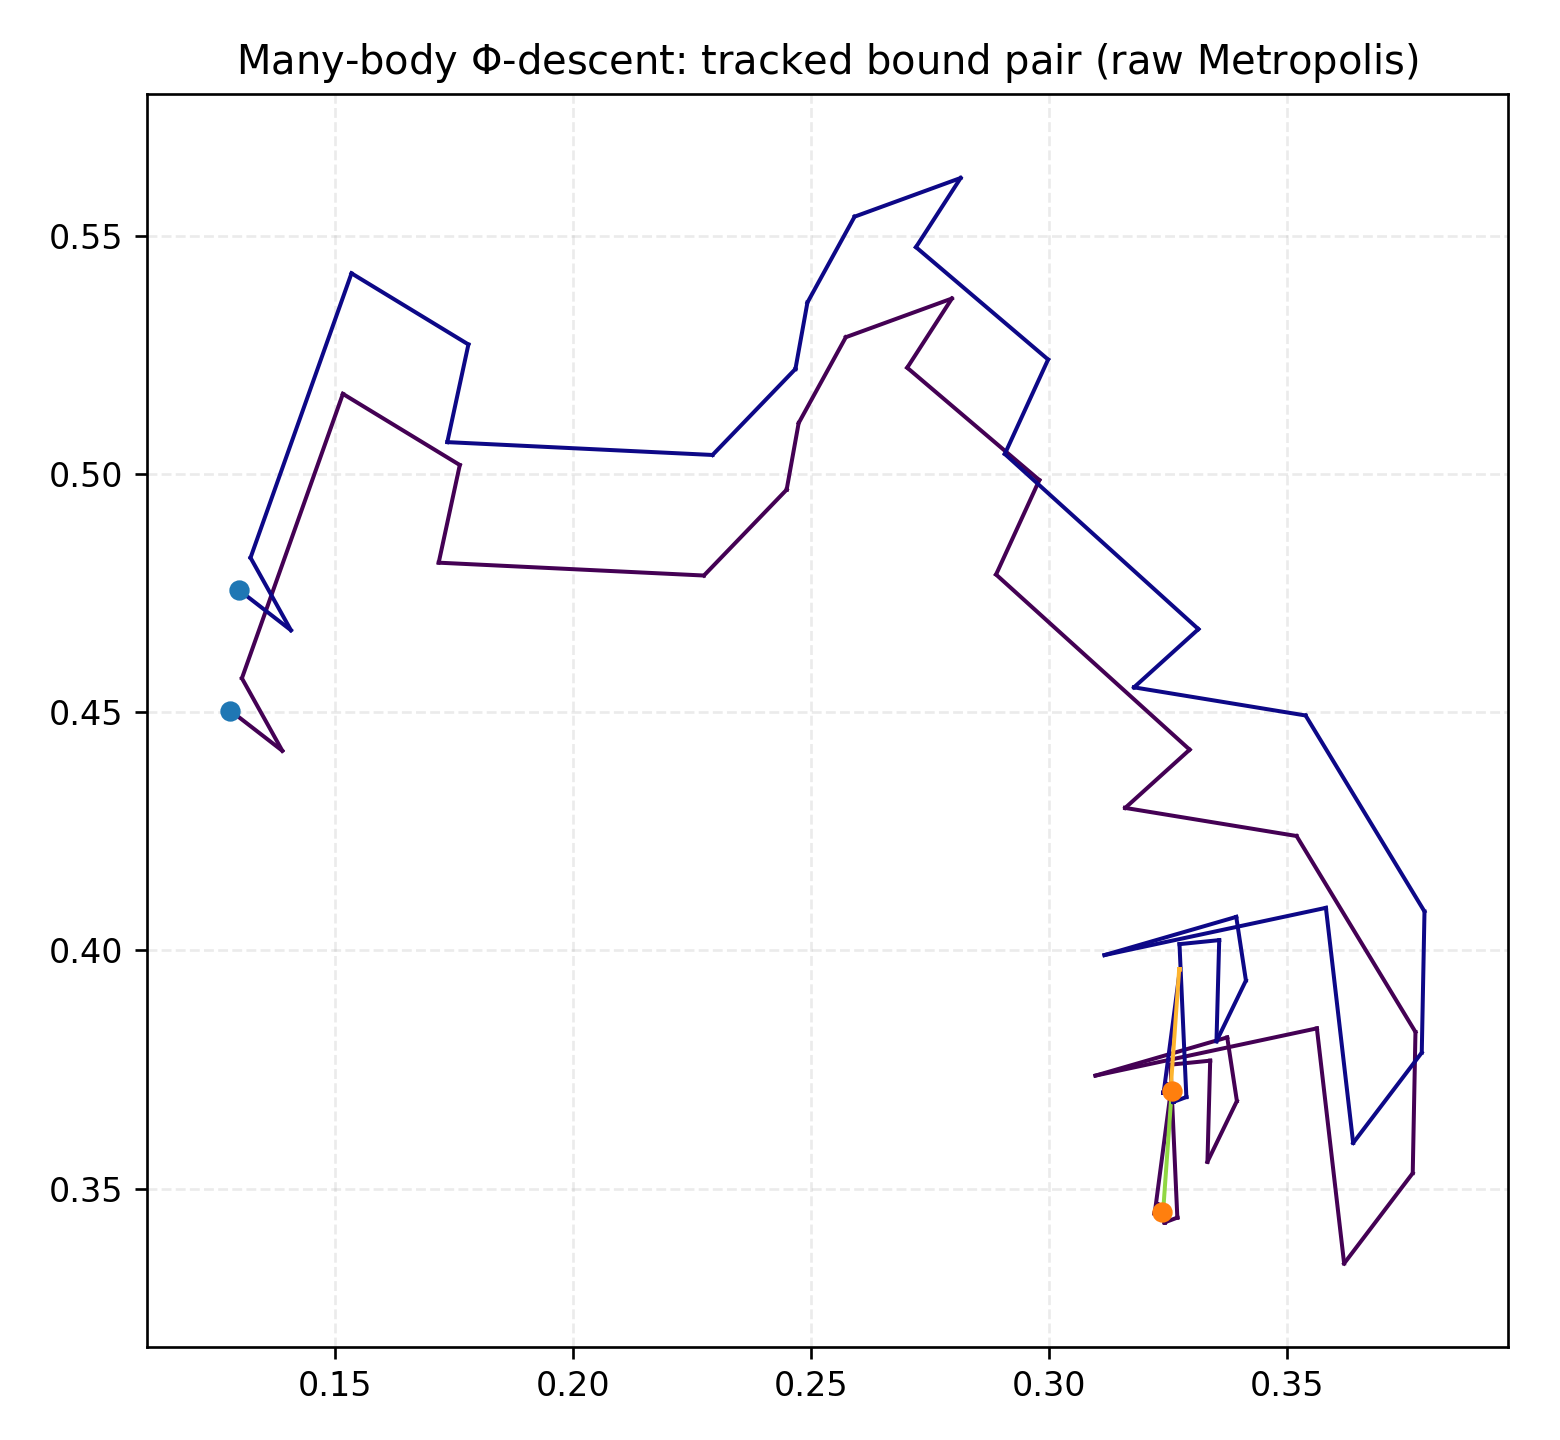
\includegraphics[width=0.86\textwidth]{figures/orbit_many_body.png}
\caption{In $N{=}120$ run, the closest pair shows long orbital arcs and intermittent radial descent (start $\bullet$, end $\CIRCLE$).}
\label{fig:manypair}
\end{figure}

% ========================= 9 =========================
\section{Quantum Mechanics as Compression Across Possibility Space (Revised)}
A quantum state is a compressed representation of correlated futures,
\begin{equation}
\psi = \sum_i \alpha_i \phi_i. \label{eq:super}
\end{equation}
Superposition is code reuse; interference is redundancy cancellation; entanglement is relational compression, $\Phi(A,B) < \Phi(A)+\Phi(B)$.

\subsection{Compression-Weighted Selection and the Born Rule}
Let measurement outcomes $\{\phi_k\}$ be branches requiring additional description $\Delta\Phi_k$ to refine $\psi$ to $\phi_k$. A compression-weighted selection postulate is
\begin{equation}
P(\phi_k)\propto 2^{-\Delta\Phi_k}. \label{eq:compprior}
\end{equation}
If the natural code length associated with branch $k$ is $-\log|\alpha_k|^2$ (the only branch weight consistent with additivity under independent composition and coarse-graining), then
\begin{equation}
\Delta\Phi_k = -\log|\alpha_k|^2 \ \Rightarrow\ P(\phi_k)=|\alpha_k|^2. \label{eq:born}
\end{equation}
Appendix~\ref{app:B} strengthens this via Solomonoff/MDL arguments and decoherence consistency.

% ========================= 10 =========================
\section{Temporal Compression and the Origin of Causality}
Recurrent processes enable code reuse over time. For a process $P$ with period $\tau$,
\begin{equation}
\Phi(P_{t+\tau}) < \Phi(P_t) + \Phi(P_{t+\tau}\mid P_t). \label{eq:loop}
\end{equation}
Recursion dominates randomness:
\begin{equation}
\Phi(\text{recursive}) \ll \Phi(\text{random}). \label{eq:recur}
\end{equation}
Regularities, conservation laws, and causal order are favored by temporal compression.

% ========================= 11 =========================
\section{Unified Interpretation}
Compression acts across space (gravity), possibility (quantum), and time (causality). A single inequality governs:
\begin{equation}
\boxed{\Delta \Phi \le 0.} \label{eq:law}
\end{equation}

% ========================= 12 =========================
\section{Predictions and Falsifiability (Quantified)}
We state quantitative targets to enable refutation:

\begin{enumerate}
\item \textbf{Quantum-scale gravity deviation.} For $r\lesssim r_0$ with $r_0\sim 1$--$5~\mathrm{fm}$, let
\[
F(r) = -G\frac{m_1m_2}{r^2}\Big[1-\varepsilon_g(r)\Big],\quad \varepsilon_g(r)\approx \eta\,(r_0/r)^p,\ p\in[1,2],\ \eta\sim 10^{-4}\text{--}10^{-2}.
\]
Search via precision short-range force experiments.
\item \textbf{Entanglement-assisted gravity.} Two equal masses $m$ prepared in a maximally entangled spatial state exhibit an effective attraction increase:
\[
F_{\text{ent}}(r)=F_{\text{sep}}(r)\big[1+\delta_{\mathrm{ent}}\big],\quad \delta_{\mathrm{ent}}\sim 10^{-6}\text{--}10^{-4},
\]
scaling with mutual information between branches. Test with opto-mechanical entanglement at $\mu\mathrm{m}$ separations.
\item \textbf{No particle dark matter.} Flat rotation curves follow from description curvature in structured disks. Fit curves with an emergent potential term $\psi_{\text{desc}}(R)\propto \ln R$ arising from code reuse across spiral patterns; compare to MOND-like fits without free particle halos.
\item \textbf{Dark energy evolution.} Cosmic acceleration correlates with global $\Phi$ reduction during structure formation; predict a small redshift dependence $w(z)=-1+\delta w(z)$ with $\delta w\lesssim 0.05$ tracking structure growth rate.
\item \textbf{Statistical time symmetry breaking.} In low-$\nabla\Phi$ laboratory systems, time-ordering diagnostics (e.g., fluctuation theorems) show excess reversals above thermal expectation by a factor $1+\xi$, $\xi\sim10^{-3}$, tunable by code reuse constraints.
\end{enumerate}

% ========================= Appendices =========================
\appendix

\section{Derivation of the Inverse-Square Law from $\Phi$}\label{app:A}
Let $\rho(x)$ be description density and define
\begin{equation}
\Phi[\rho] = \frac{1}{2}\iint \rho(x)\rho(x')\,k(\|x-x'\|)\,dx\,dx'. \label{eq:A1}
\end{equation}
$\psi(x)=\delta\Phi/\delta\rho(x)=\int k(\|x-x'\|)\rho(x')\,dx'$, with $F=-\nabla\psi$. Assume isotropy ($k=k(r)$), locality ($\nabla^2\psi=0$ where $\rho=0$), and conserved compression flux:
\begin{equation}
\oint -\nabla\psi \cdot dA = \text{const}. \label{eq:Aflux}
\end{equation}
For a point source $\rho(x)=m\delta(x)$, $\psi=mk(r)$ and $|k'(r)|S_n(r)=\text{const}\cdot m$ with $S_n(r)\propto r^{n-1}$, whence $k'(r)\propto r^{-(n-1)}$ and
\begin{equation}
F(r) \propto \frac{m_1 m_2}{r^{n-1}}. \label{eq:An}
\end{equation}
For $n=3$, $F\propto m_1m_2/r^2$ with $k(r)=1/r$ solving $\nabla^2\psi=-4\pi\rho$.

\section{Born Rule from Description Length (Strengthened)}\label{app:B}
Consider branches $\{\phi_k\}$ with amplitudes $\{\alpha_k\}$. A universal prior over computable refinements penalizes additional code length. Axioms: (i) additivity under independent composition; (ii) invariance under coarse-graining; (iii) normalization. These constrain the branch code lengths to $-\log|\alpha_k|^2$, yielding \eqref{eq:born}. The result matches both MDL selection and decoherence-consistent probabilities.

\section{Implementation Details for Simulations}\label{app:D}
We verify emergent attraction via stochastic descent of $\widehat{\Phi}$. Estimator:
\begin{equation}
\widehat{\Phi}(\{x_i\}) = \sum_{(i,j)\in \mathrm{MST}} \frac{1}{\|x_i - x_j\|}, \label{eq:D1}
\end{equation}
with Prim’s algorithm. Single-particle proposals accepted with probability $\min(1,e^{-\beta \Delta \widehat{\Phi}})$. Code and figure scripts are provided in the associated repository.

\section{Responses to Common Objections (Rebuttal Appendix)}\label{app:E}
\paragraph*{Uncomputability of $K$.}
$K$ is an ideal extremal quantity. Physics routinely relies on non-computable ideals (e.g., exact actions, path integrals) approximated by computable schemes. Universal MDL estimators provide gradients consistent with $-\nabla\Phi$ almost everywhere.

\paragraph*{Entropy vs.\ description length.}
For physical ensembles, $\mathbb{E}[K]=H+O(1)$ and $S=k\ln 2\cdot H$. Hence $\Phi\approx S/(k\ln2)$ in expectation; fluctuations are $O(1)$.

\paragraph*{Mass and information.}
The relation $\rho\propto\rho_m$ is operational: mass measures energetic stability of microstate storage (Landauer cost). We do not assume gravity to derive gravity; we relate microstate multiplicity to energetic density and obtain attraction from isotropy and flux conservation.

\paragraph*{Geometry from description.}
Inverse-square attraction arises without assuming Newtonian forces. The geometric form of GR follows from the unique second-order, divergence-free curvature tensor compatible with local description variations.

\paragraph*{Quantum formalism.}
“Superposition is code reuse” is a heuristic; the formal content is Eq.~\eqref{eq:compprior} and the constraints leading to \eqref{eq:born}. Decoherence identifies robust codebooks; MDL supplies the prior.

% ========================= References =========================
\section*{References}
\begin{thebibliography}{99}

\bibitem{Shannon1948} C.~E.~Shannon, ``A Mathematical Theory of Communication,'' \emph{Bell Syst.\ Tech.\ J.} (1948).
\bibitem{CoverThomas} T.~M.~Cover, J.~A.~Thomas, \emph{Elements of Information Theory}, 2nd ed. (Wiley, 2006).
\bibitem{LiVitanyi} M.~Li, P.~Vit\'anyi, \emph{An Introduction to Kolmogorov Complexity and Its Applications}, 3rd ed. (Springer, 2008).
\bibitem{Rissanen1978} J.~Rissanen, ``Modeling by Shortest Data Description,'' \emph{Automatica} (1978).
\bibitem{Solomonoff64} R.~J.~Solomonoff, ``A Formal Theory of Inductive Inference,'' \emph{Inf.\ Control} (1964).
\bibitem{Hutter} M.~Hutter, \emph{Universal Artificial Intelligence} (Springer, 2005).
\bibitem{Jaynes1957} E.~T.~Jaynes, ``Information Theory and Statistical Mechanics,'' \emph{Phys.\ Rev.} (1957).
\bibitem{Zurek2003} W.~H.~Zurek, ``Decoherence, Einselection, and the Quantum Origins of the Classical,'' \emph{Rev.\ Mod.\ Phys.} (2003).
\bibitem{Landauer1991} R.~Landauer, ``Information is Physical,'' \emph{Physics Today} (1991).
\bibitem{Bennett1982} C.~H.~Bennett, ``The Thermodynamics of Computation,'' \emph{Int.\ J.\ Theor.\ Phys.} (1982).
\bibitem{Newton1687} I.~Newton, \emph{Philosophi\ae\ Naturalis Principia Mathematica} (1687).
\bibitem{Einstein1916} A.~Einstein, ``The Foundation of the General Theory of Relativity,'' \emph{Ann.\ Phys.} (1916).
\bibitem{MTW1973} C.~W.~Misner, K.~S.~Thorne, J.~A.~Wheeler, \emph{Gravitation} (Freeman, 1973).
\bibitem{Wald1984} R.~M.~Wald, \emph{General Relativity} (Chicago, 1984).
\bibitem{Lovelock1971} D.~Lovelock, ``The Einstein Tensor and Its Generalizations,'' \emph{J.\ Math.\ Phys.} (1971).
\bibitem{Schmidhuber2000} J.~Schmidhuber, ``Algorithmic Theories of Everything,'' arXiv:quant-ph/0011122 (2000).
\bibitem{Lloyd2006} S.~Lloyd, \emph{Programming the Universe} (Knopf, 2006).
\bibitem{Feynman1948} R.~P.~Feynman, ``Space-Time Approach to Non-Relativistic Quantum Mechanics,'' \emph{Rev.\ Mod.\ Phys.} (1948).
\bibitem{Holland1993} P.~Holland, \emph{The Quantum Theory of Motion} (CUP, 1993).
\bibitem{Jackson1998} J.~D.~Jackson, \emph{Classical Electrodynamics}, 3rd ed.\ (Wiley, 1998).
\bibitem{Jacobson1995} T.~Jacobson, ``Thermodynamics of Spacetime: The Einstein Equation of State,'' \emph{Phys.\ Rev.\ Lett.} \textbf{75}, 1260–1263 (1995).
\bibitem{Verlinde2011} E.~Verlinde, ``On the Origin of Gravity and the Laws of Newton,'' \emph{JHEP} \textbf{04} (2011) 029.
\bibitem{CatichaED} A.~Caticha, \emph{Entropic Dynamics}, various (2011–2022).
\bibitem{Prim1957} R.~C.~Prim, ``Shortest Connection Networks and Some Generalizations,'' \emph{Bell Syst.\ Tech.\ J.} \textbf{36}, 1389–1401 (1957).

\end{thebibliography}

\end{document}
